\documentclass[11pt,a4paper]{ctexart}

\usepackage[margin=2.6cm]{geometry}
\usepackage{amsmath,amssymb,amsthm}
\usepackage{graphicx}
\usepackage{booktabs}
\usepackage{hyperref}
\usepackage{xcolor}
\usepackage{listings}
\usepackage{caption}

\graphicspath{{figures/}}
\hypersetup{colorlinks=true, linkcolor=blue!50!black, urlcolor=blue!60!black}
\lstset{
  basicstyle=\ttfamily\small,
  breaklines=true,
  frame=single,
  columns=fullflexible,
  backgroundcolor=\color{gray!7}
}

\newtheorem{definition}{定义}[section]
\newtheorem{theorem}{定理}[section]
\newtheorem{lemma}{引理}[section]
\newtheorem{proposition}{命题}[section]
\newtheorem{example}{例}[section]

\title{附录 A \quad Background / 背景知识}
\author{基于 \textit{A Course in Time Series Analysis} 的中文讲义与 Python 实践}
\date{}

\begin{document}
\maketitle

\section*{本章学习目标}

本章按照原文 \textit{Background} 的小节顺序整理，保留主要定义、定理、模型公式和练习方向，并将原文中的 R 实践思路改写为 Python 工程实践。

完成本章后，应能够：
\begin{itemize}
  \item 复习常用不等式和概率收敛工具；
  \item 理解鞅差和 Burkholder 不等式；
  \item 掌握 Fourier 级数和正交展开；
  \item 理解 FFT 的分治思想；
  \item 为正文中的渐近证明和频域计算提供背景。
\end{itemize}

\section{定义与不等式}

附录首先整理概率界和矩不等式。常用工具包括 Markov 不等式、Chebyshev 不等式、Cauchy-Schwarz 不等式和 Jensen 不等式。例如
\[
  P(|X|>\epsilon)\le \frac{E|X|^p}{\epsilon^p}.
\]

\begin{lemma}[原文 Lemma A.1.1]
若随机变量或随机过程满足给定矩界，则可用最大不等式控制其上确界或部分和，从而推出收敛率。
\end{lemma}

\begin{theorem}[Helly 定理，原文 Theorem A.1.1]
分布函数序列若紧，则存在弱收敛子序列。该结果用于分布收敛的紧性论证。
\end{theorem}

\section{鞅}

\begin{definition}[鞅差，原文 Definition A.2.1]
若 \(E(X_t\mid\mathcal F_{t-1})=0\)，则 \(\{X_t\}\) 关于过滤 \(\{\mathcal F_t\}\) 为鞅差序列。
\end{definition}

鞅差是时间序列渐近理论中的核心对象。许多估计方程可分解为鞅差和小余项，然后用鞅中心极限定理或最大不等式处理。

\section{Fourier 级数}

周期函数可展开为
\[
  f(x)=a_0+\sum_{k=1}^{\infty}\{a_k\cos(kx)+b_k\sin(kx)\}.
\]
复指数形式为
\[
  f(x)=\sum_{k=-\infty}^{\infty}c_ke^{ikx},
  \qquad
  c_k=\frac1{2\pi}\int_{-\pi}^{\pi}f(x)e^{-ikx}\,dx.
\]
正文中的谱密度、DFT 和周期检测都建立在这一正交展开思想上。

\section{Burkholder 不等式与 FFT}

\begin{theorem}[Burkholder 不等式，原文 Theorem A.4.1--A.4.2]
对鞅差部分和 \(S_n=\sum_{t=1}^nY_t\)，其 \(p\) 阶矩可由条件方差和单项矩控制。该工具用于证明时间序列估计中的最大界和收敛率。
\end{theorem}

\section{快速 Fourier 变换}

DFT 定义为
\[
  d(\omega_j)=\sum_{t=0}^{n-1}x_t e^{-i2\pi jt/n}.
\]
当 \(n=2m\) 时，可把偶数项和奇数项分开：
\[
  d_n(j)=d_m^{(even)}(j)+e^{-i2\pi j/n}d_m^{(odd)}(j),
\]
从而递归计算，把复杂度从 \(O(n^2)\) 降到 \(O(n\log n)\)。

\section{Python 工程实践}

在本章目录下运行：
\begin{lstlisting}[language=bash]
python scripts/appA_generate_figures.py
\end{lstlisting}

脚本会把图像写入本章 \texttt{figures/} 目录。当前图像用于配合本章核心概念的仿真说明；若后续补齐原始数据文件，可把模拟数据替换为原文真实数据案例。

\begin{figure}[htbp]
  \centering
  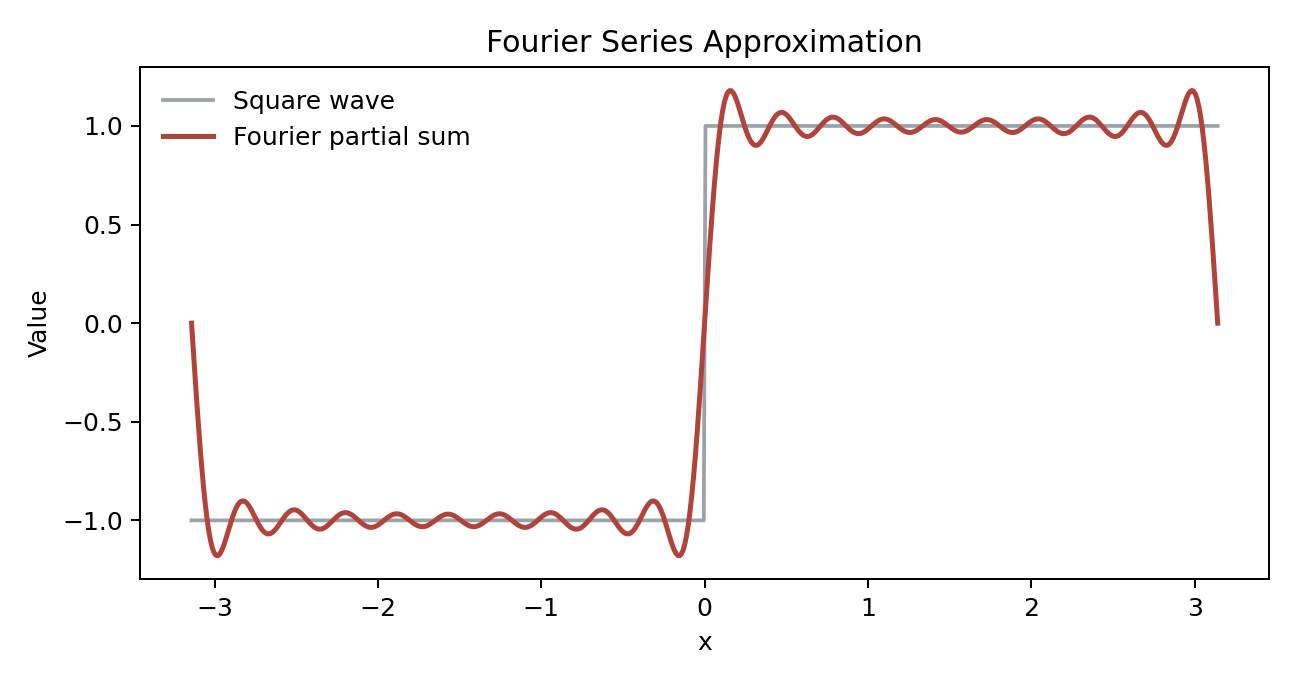
\includegraphics[width=0.86\textwidth]{appA_fig01_fourier_series.png}
  \caption{Fourier 级数近似：用有限个正弦项逼近方波。}
\end{figure}

\begin{figure}[htbp]
  \centering
  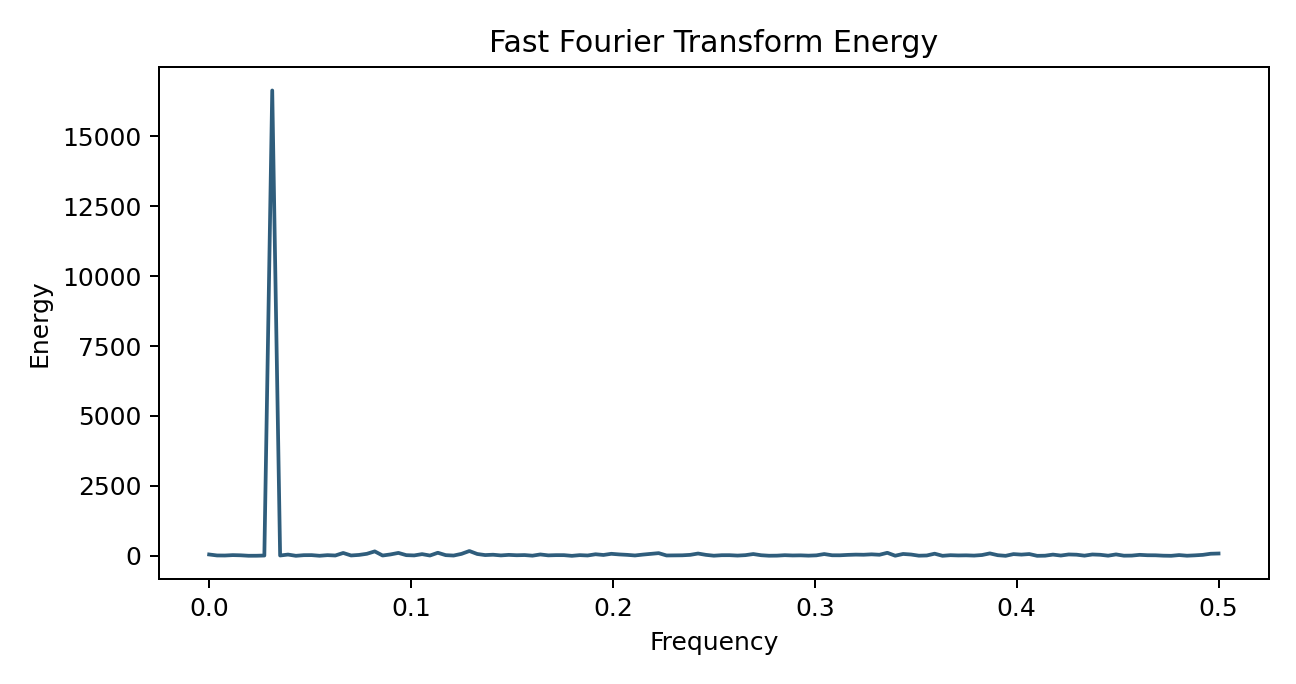
\includegraphics[width=0.86\textwidth]{appA_fig02_fft_energy.png}
  \caption{FFT 能量示例：快速 Fourier 变换用于高效计算频域能量。}
\end{figure}

\section{练习提要}

原文练习主要围绕下列方向展开：
\begin{itemize}
  \item 用 Markov 和 Chebyshev 不等式证明简单概率界；
  \item 验证鞅差的条件期望为 0；
  \item 计算简单周期函数的 Fourier 系数；
  \item 手推 \(n=4\) 时 FFT 的偶奇分解。
\end{itemize}

\section*{本章小结}

附录 A 收集正文所需的概率和分析工具。鞅不等式支撑渐近证明，Fourier 级数和 FFT 支撑频域表示与计算。

\end{document}
